\chapter{Contexto}
\label{chap:Chapter2}

\textit{A definir}

\section{A Empresa}
\label{sec:chap2_company}

A {\companyname} é uma empresa fundada em 2009, com sede e centro de engenharia na Maia (Porto, Portugal), subsidiárias em Dresden (Alemanha), Suzhou (China), Austin (Estados Unidos da América) e um escritório comercial em Taiwan. O objetivo é proporcionar à indústria uma solução de gestão e controlo de produção, procurando reduzir os custos de produção, flexibilizar para satisfazer a procura e capacitar a organização de uma maior agilidade, visibilidade e fiabilidade~\parencite{cmf_overview}. O compromisso da empresa~\parencite{cmf_overview} foca-se no desenvolvimento de~\inquotes{soluções de vanguarda, indo de encontro aos desafios mais importantes da indústria e disponibilizar à lista crescente de clientes satisfeitos, soluções de elevado valor acrescentado, no prazo e orçamento requerido}\footnote{Tradução livre do autor. No original~\inquotes{[...] solutions that address the most urgent industry challenges and provide our growing list of satisfied customers with the highest value solution, on-time and on-budget.}.}.

A estratégia da empresa está sintetizada na sua missão, visão e valores. Se a missão descreve a razão da empresa existir, ou seja, o seu propósito, já a visão retrata o que se aspira alcançar~\parencite[pp.~65-66]{mission_vision_values_what_do_they_say}. Isto posto, a missão e visão são divulgados a seguir~\parencite{cmf_strategy}: 

\begin{itemize}
    \item 
    {
        \textit{Missão} -- \inquotes{Trazer valor através da convergência de inteligência, operações e tecnologias de automação para a Indústria 4.0.}\footnote{Tradução livre do autor. No original \inquotes{We drive business value through the convergence of intelligence, operations, and automation technologies for Industry 4.0.}.}.
    }
    \item 
    {
        \textit{Visão} -- \inquotes{Tornar a Indústria 4.0 uma realidade para todos fabricantes.}\footnote{Tradução livre do autor. No original \inquotes{We will make Industry 4.0 a reality for all manufacturers.}.}.
    }
\end{itemize}

Relativamente aos valores, são estes que suportam a visão, moldam a cultura empresarial e são a essência da sua identidade. Como tal, de seguida apresentam-se os valores da Critical Manufacturing~\parencite{cmf_strategy}:

\begin{itemize}
    \item 
    {
        \textit{Inovação} -- \inquotes{Exceder as expectativas dos clientes através das soluções mais eficientes e de mais alto valor para indústria.}\footnote{Tradução livre do autor. No original \inquotes{We constantly exceed our customers’ expectations through the most efficient and high value-added manufacturing solutions.}.}.
    }
    \item
    {
        \textit{Agilidade} -- \inquotes{Adaptar as pessoas, processos e soluções de forma a responder à evolução do mundo da manufatura de alta tecnologia.}\footnote{Tradução livre do autor. No original \inquotes{We continuously adapt our people, processes and solutions to respond to the evolving world of high-tech manufacturing.}.}.
    }
    \item
    {
        \textit{Compromisso} -- \inquotes{Defender o sucesso contínuo dos clientes e da empresa.}\footnote{Tradução livre do autor. No original \inquotes{We champion the continued success of our customers and our company.}.}.
    }
\end{itemize}

Por conseguinte, com base na sua estratégia, o presente trabalho pretende demonstrar viabilidade e o valor da utilização da \gls{IA}, nomeadamente na área do \gls{PLN}, para a interação com o {\productname} e obter informação pertinente para o utilizador final. 

\section{O Produto}
\label{sec:chap2_product}

Nos últimos anos, o mercado dos sistemas de informação empresariais tem vindo a crescer, sobretudo pela necessidade das empresas aumentarem a sua produtividade e consequentemente, melhorarem a sua competitividade. Embora sistemas \gls{ERP} sejam cada vez mais usuais nas empresas, no sentido de gerir as suas operações, estes falham quando aplicados num contexto fabril, ou seja, no \inquotes{chão de fábrica}. Os departamentos produtivos beneficiam de \textit{software} personalizado, que responda às necessidades específicas do foro produtivo/industrial~\parencite{mes_literature_review}. 

Nestas circunstâncias surge o conceito de \gls{MES}, fruto da necessidade das empresas de manufatura progredirem no mercado, num ponto de vista de melhoria da reatividade, da qualidade, dos custo de produção e dos prazos de entrega. Desse modo, as funções de um \gls{MES} estão sobretudo ligadas a atividades de manufatura, que representa uma parte substancial do valor acrescentado em empresas deste setor~\parencite{mes_literature_review}. 

Com o objetivo de apresentar o produto, nesta secção faz-se um enquadramento genérico do conceito \gls{MES} e posteriormente, foca-se o caso específico do {\productname}.

\subsection{\textit{Manufacturing Execution Systems}}

A organização MESA\footnote{Manufacturing Enterprise Solutions Association. \url{http://www.mesa.org}}, uma comunidade mundial, sem fins lucrativos, que junta empresas de manufatura, de prestação de serviços, analistas, académicos e estudantes, com o propósito de melhorar os resultados do negócio e as operações de produção, através da implementação e implantação de tecnologias de informação e das melhores práticas de gestão, deu o primeiro passo na definição formal de \gls{MES}~\parencite{mes_explained_high_level_vision}:

\begin{quote}
    \inquotes{\textit{Os Manufacturing Execution Systems (MES) fornecem informações que possibilitam a otimização de atividades de produção, desde o lançamento do pedido até aos produtos acabados. Usando dados atualizados e precisos, o MES orienta, inicia, responde e relata as atividades da fábrica à medida que elas ocorrem. A resposta rápida, resultante das mudanças nas condições, associada ao foco na redução de atividades sem valor acrescentado, impulsiona a eficácia das operações e processos fabris. O MES melhora o retorno dos ativos operacionais, bem como o prazo de entrega, gestão de stock, margem bruta e desempenho do fluxo de caixa. O MES fornece informações críticas acerca das atividades de produção em toda a empresa e cadeia logística através de comunicações bidirecionais.}}\footnote{Tradução livre do autor. No original \inquotes{Manufacturing Execution Systems (MES) deliver information that enables the optimization of production activities from order launch to finished goods. Using current and accurate data, MES guides, initiates, responds to, and reports on plant activities as they occur. The resulting rapid response to changing conditions, coupled with a focus on reducing non value-added activities, drives effective plant operations and processes. MES improves the return on operational assets as well as on-time delivery, inventory turns, gross margin, and cash flow performance. MES provides mission-critical information about production activities across the enterprise and supply chain via bi-directional communications.}.}.
\end{quote}

Portanto, o sistema \gls{MES} age como um intermediário entre os diversos processos existentes no \inquotes{chão de fábrica} e os sistemas de \inquotes{alto nível}, existindo comunicação bidirecional entre as camadas, como se demonstra na Figura~\ref{fig:mes_layers}. O \gls{MES} tanto pode fornecer informação acerca dos custos de produção, de indicadores de \textit{performance}, do estado das ordens de fabrico ou rendimento produtivo, como pode também obter dados sobre o planeamento das atividades fabris, parâmetros operacionais, receitas ou instruções de fabrico, por forma a inferir de forma inteligente sobre a fábrica e os seus processos~\parencite{mes_explained_high_level_vision}.

\begin{figure}[!ht]
    \centering
    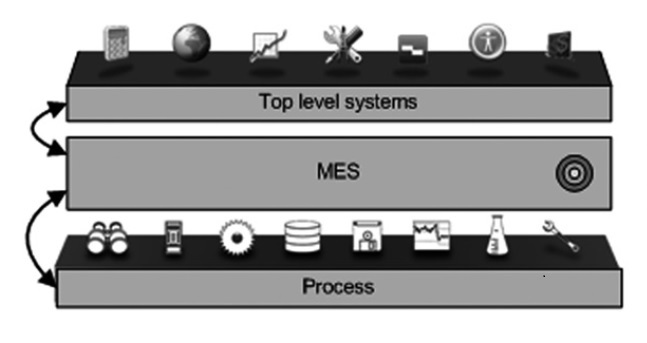
\includegraphics[width=.75\textwidth]{ch2/assets/mes_layers.jpg}
    \caption{Ambiente \gls{MES} e as suas camadas, baseado em~\textcite[p.~526]{mes_literature_review}.}
    \label{fig:mes_layers}
\end{figure}

Com o intuito de dar resposta às necessidades de diversos ambientes produtivos, as funções apresentadas de seguida são essenciais para um \gls{MES}~\ref{fig:mes_functions}

\begin{figure}[!ht]
    \centering
    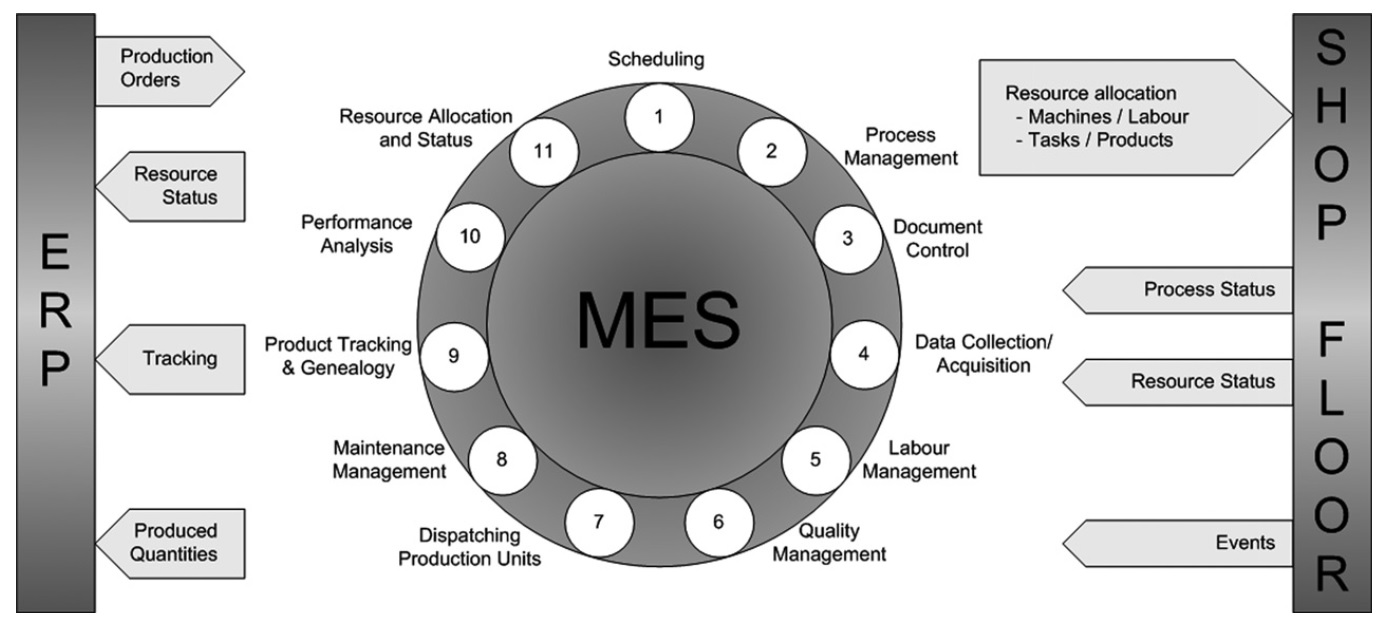
\includegraphics[width=\textwidth]{ch2/assets/mes_functions.jpg}
    \caption{bla}
    \label{fig:mes_functions}
\end{figure}


\subsection{\textit{{\productname}}}

\section{Análise de Valor}
\label{sec:chap2_valueanalysis}

\textit{A definir}